%
% 2drand.tex
%
% (c) 2024 Prof Dr Andreas Müller
%
\begin{figure}
\centering
\vspace*{2cm}
XXX Rand eines zweidimensionalen Gebietes
\vspace*{2cm}
%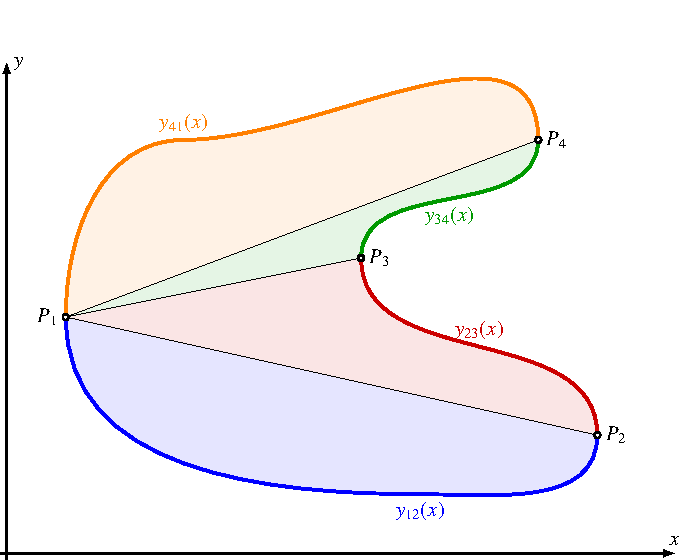
\includegraphics{chapters/040-felder/images/2drand.pdf}
\caption{Der Rand eines zweidimensionalen Gebietes mit glattem Rand
kann stückweise als Graphen von Funktion $y_k(x)$ beschrieben werden.
\label{buch:felder:fundamentallemma:fig:2drand}}
\end{figure}
